%!TEX root = main.tex
\chapter{Background}

\section{Computer supported reflection}
Reflection is critical to workplace learning, enabling employees to make sense of complex and dynamic situations\cite{Schon1983}. Boud et al.\cite{boudreflection1985} defined learning through reflection as “those intellectual and affective activities in which individuals engage to explore their experiences in order to lead to new understandings and appreciations.”
The MIRROR project describes reflective learning as the conscious re-evaluation of experience for the purpose of guiding future behavior, acknowledging the need to attend to feelings, ideas as well as behavior associated with work experience\cite{krogstiemodel}.
Work and reflection on this work are heavily connected\cite{Schon1983}, both driving each other forward. Experiences are created through work, and these experiences can be reflected upon. Reflection can be based on both a memory of an experience, and on data from the experience. Revisiting and reflecting on a work experience leads to a better understanding of the experience and allows for learning from it. Reflection can help developers learn from experiences and gain knowledge of how to deal with work-related challenges. This relationship between reflection and learning has been modeled as an experience-based learning cycle\cite{Korthagen_Vasalos_2005, KolbModel}.
Reflection has both individual and social dimensions[ref 8,9]. Social wise reflection is often performed collaboratively by teams performing a joint task, and therefore shares some common ground and experience. 

Most reflective learning in a work environment, happens analogically without support of technology[ref 13]. Technology has been shown to increase the potency of reflection and reflective learning at work [ref 14-19].
MIRROR[20] presents a reflection-learning cycle [\ref{CSRL cycle model og 20 }. One key part of this model is the reflection session. These sessions is where the team gathers and actively reflects on experiences, both informal or formal. 

\subsection{The MIRROR model}
The MIRROR model off Computer Supported Reflective Learning (CSRL), is a work on how to incorporate reflection in to the daily routine at work.

\begin{figure}[!htpb]
\label{logo}
\centering
	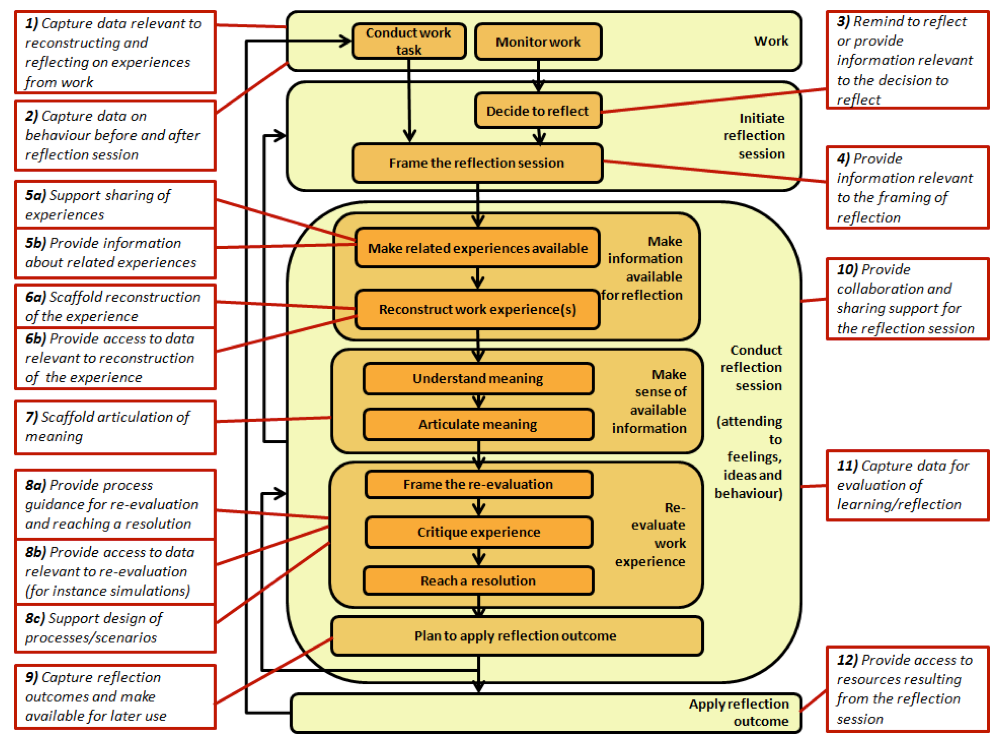
\includegraphics[width=0.8\textwidth]{mirror}
\caption{MIRROR model}
\end{figure}

In the model presented in \ref{logo}, Boud et.al [7] presents reflection as a
process with several steps without any fixed sequence. The major theme in
the model is that experience is what is reflected upon, including the behavior,
feelings and ideas connected to that experience. In the reflective process
you return to the experience, attend to connected feelings and re-evaluate
the experience. In the model, an iteration between the experience and reflections
is indicated, meaning that the reflective process and the experience
can intervene before the outcome becomes clear. The outcome then consists
of new perspectives, changes in the behavior, readiness for application
and commitment to action. All the steps of the process does not need to
be included to achieve an instance of reflection, but they are guidelines for
understanding the reflective process.
In this thesis we utilize this model by trying to capture the events in the
experience, as a snapshot in the timeline. This will make it easier to return
to the experience and reflect. The challenge will be to capture the ideas,
behavior and feelings that is involved in the experience and using technology
to support the reflective process.

%\subsection{Birgits PHD}
% PhD: http://www.idi.ntnu.no/research/doctor_theses/birgitkr.pdf  .

\section{Agile Software Development}
Theoretical background about agile development. Normaly a project is divided into milestones, these milestones will then again be divided into issues and weighted on how much work is required to finish working on each of them.\linebreak
\emph{Manifesto for Agile Software Development:}\cite{agilemanifesto}
\begin{quotation}
We are uncovering better ways of developing software by doing it and helping others do it. Through this work we have come to value:
\begin{itemize}
\item Individuals and interactions over processes and tools
\item Working software over comprehensive documentation
\item Customer collaboration over contract negotiation
\item Responding to change over following a plan
\end{itemize}
That is, while there is value in the items on
the right, we value the items on the left more.\\*
\end{quotation}

\begin{figure}[!htpb]
\label{logo}
\centering
	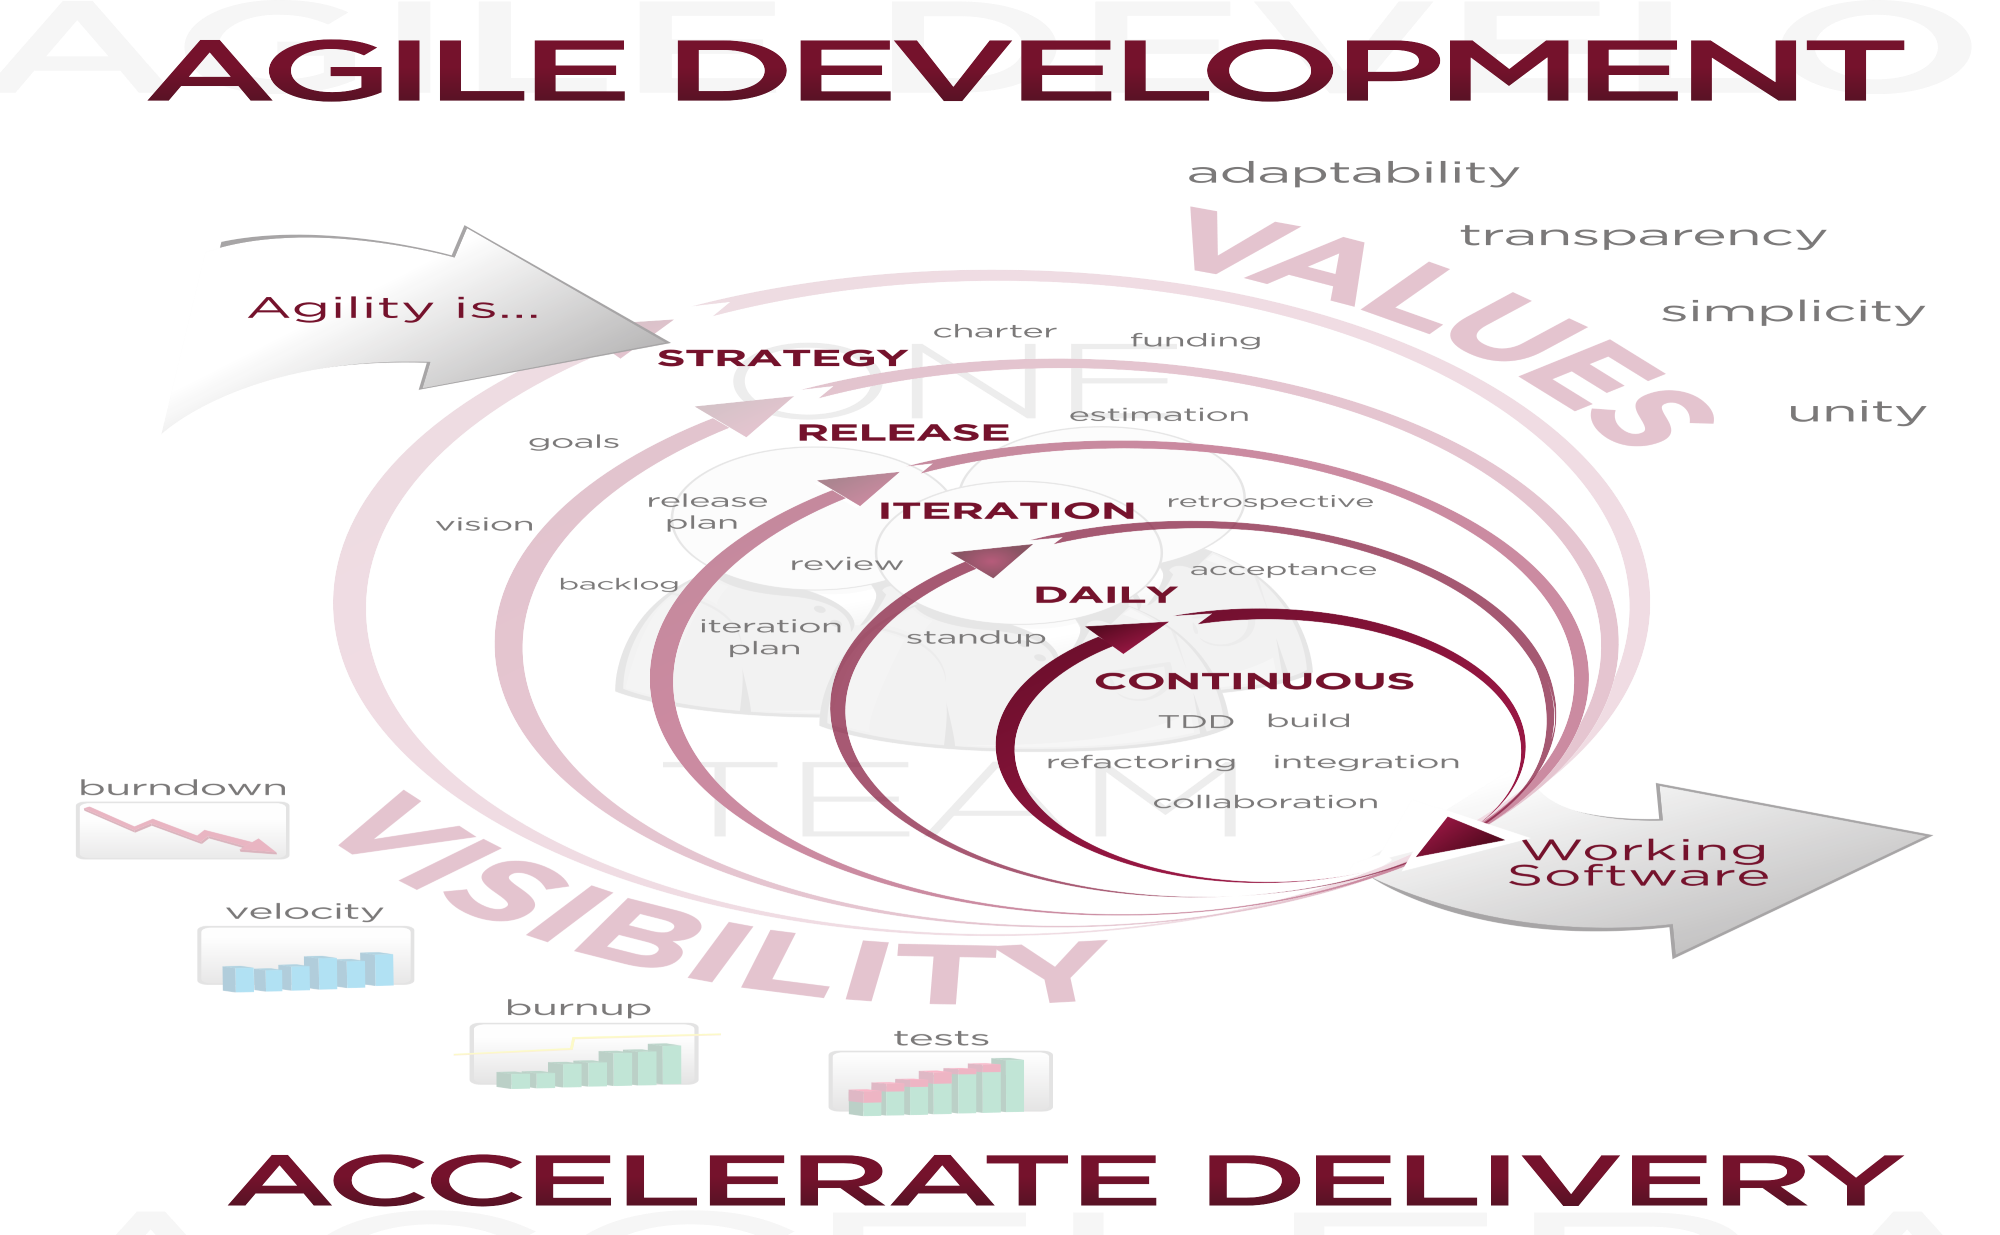
\includegraphics[width=0.8\textwidth]{agile_model}
\caption{Agile software development poster}
\end{figure}

The poster above represents the different iterations a team of developeres iterates through when using agile development meothodology.

\subsection{Scrum}
Scrum is a type of agile development, it has set intervalls(normally 2 to 4 weeks) for each milestone with each milestone containing about the same amount of work.

\begin{figure}[!htpb]
\label{logo}
\centering
	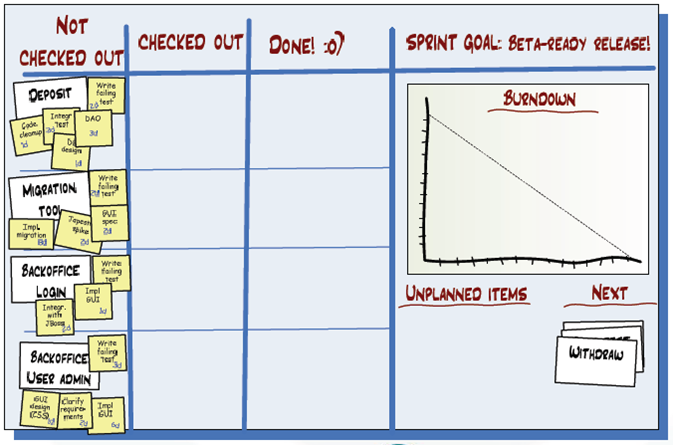
\includegraphics[width=0.8\textwidth]{scrumboard}
\caption{Example of scrum board}
\end{figure}

A scrumboard as shown above is used for each milestone to show which issues have been started on and who is working on which feature. The chart to the right is a burndown chart, stating how many hours the team has to work inorder to complete on time.